\chapter{Application}\label{chap:application}

\newcommand{\download}{Download\xspace}
\newcommand{\live}{Live\xspace}
\newcommand{\serviceprovisioning}{Provisioning\xspace}
\newcommand{\streaming}{Streaming\xspace}

While the previous chapter focussed on the network and the impact of applications, vendors, and users thereon, this chapter shifts focus on the applications.
The Internet supports a multitude of different applications, including video streaming services, online gaming, file storage services, cloud office solutions, and uncountable more.
%cite? cisco vni?
In this chapter, we focus on two of the most prominent application types: Video streaming and file storage, chosen due to their impact on global traffic and frequency of use.
In contrast to applications of earlier generations, todays services are not standardised or under control by network operators but rather the result of free enterprise and enterpreneurship.
While in the last chapter we were able to rely on standard documents to model the systems under study, this option is no longer available when considering applications.
Thus, we have to perform measurements or rely on studies of other researchers in order to obtain knowledge of both the systems under study as well as the related stakeholders.

Similar to \refchap{chap:network}, we identify a set of involved stakeholders and their respective key performance indicators and derive corrosponding metrics.
First, we consider the \emph{application provider}. 
In the case of the video streaming scenario, this role is realised by the video provider.
We consider the video provider to be interrested in two performance indicators: 
\begin{enumerate*}
\item user satisfaction, realised by a \gls{QoE} metric,
\item cost reduction in compute and network infrastructure, realised by the amount of traffic transmitted to a user about to abort playback.
\end{enumerate*}
In the case of the file synchronisation scenario, we consider the application operator to be interrested in user satisfaction, again realised by as \gls{QoE} metric, the mean time to synchronisation.
Wasted traffic is not of concern in this scenario, as file synchronisations are usually not aborted.
Second, we consider the \emph{network operator}.
As in the last chapter, they are interested in reducing stress on the network infrastructure.
We measure this key performance indicator by considering the number of connections to the mobile network required to complete the synchronisation operation.
Similarly to \refchap{chap:network}, we assume that the \emph{user} is interested in both a high \gls{QoE} as well long battery life for his device, represented by the energy consumption metric. 

In the current state of the art, video transmissions are considered from the perspective of the video provider or the user. 
Neither network operators nor heterogenous user profiles are considered.
Studies of file synchronisation services do not consider effects of synchronsation scheduling mechanisms on user satisfaction or energy consumption.  

The contribution of this chapter is threefold:
\begin{enumerate*}
\item We provide models for video transmission mechanisms and perform a performance evaluation and tradeoff analysis considering metrics relevant to network operators, users, and video providers.
\item We provide a \gls{QoE} model for video streaming allowing for the analysis of heterogenous user profiles and use this model in order to evaluate the impact of offered network load on video streaming scenarios.
\item We propose a model for cloud file synchronisation and evaluate a set of scheduling mechanisms regarding impact of considered metrics for all stakeholders.
\end{enumerate*}

The content from this chapter has been published in \cite{Schwartz2013b, Hossfeld2015, Schwartz2014a}.
\refsec{sec:application:background} we discuss the current state of the art regarding video transmission mechanisms and \gls{QoE} studies.
Then, in \refsec{sec:application:lte_video} we discuss tradeoffs between different video transmission mechanisms, regarding the considered metrics.
In \refsec{sec:application:qoe_user_behaviour} we study the impact of user preferences on the \gls{QoE} experienced during video streaming.
Finally, in \refsec{sec:application:cloud_file_synchronisation} we consider the impact of different file synchronisation scheduling algorithms on the relevant stakeholders.

\section{Background and Related Work}\label{sec:network:background}
This section discusses the technical background relevant to the remainder of this chapter.
First, in \refsec{sec:network:background:umts_rrc} we introduce the \gls{UMTS} mobile communication standard, and the \gls{RRC} protocol.
Then we discuss existing aproaches to measure \gls{RRC} protocol transactions and optimise the signalling load generated by \gls{RRC} messages in \refsec{sec:network:background:measurement_optimisation}.
Finally, \refsec{sec:network:background:energy_consumption_qoe} tackles smartphone power consumption and \gls{QoE}, two metrics influenced by the configuration of the \gls{RRC} protocol.

\subsection{\headershortacr{UMTS} Networks and the \headershortacr{RRC} Protocol}\label{sec:network:background:umts_rrc}
A \gls{3G} \gls{UMTS} mobile network consists of three main components, which are depicted in \reffig{fig:network:background:mobile_network_overview}: The \gls{UE}, the \gls{RAN}, and the \gls{CN}.
The \gls{RAN} is used to establish connectivity between the \gls{UE} and the \gls{CN}, which in turn can establish connectivity to the Internet, if required.

\begin{figure}
	\centering
	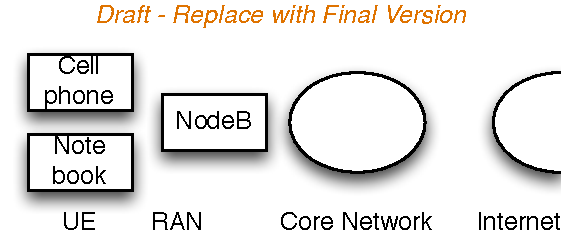
\includegraphics{network/background/figures/mobile_network_overview}
	\caption{Overview of Mobile Network}
	\label{fig:network:background:mobile_network_overview}
\end{figure}

\gls{UE} consists of devices used by end users, i.e. smartphones, tablets or data card enabled notebooks, but can also include \gls{M2M} devices.
The \gls{RAN} is, amongst other tasks, responsible for \gls{RRC}, packet scheduling and handover control.
It includes network entities such as the \gls{NodeB} and the \gls{RNC}.
The \gls{CN} provides the backbone network of the \gls{UMTS} network and provides connectivity to the Internet and the \gls{PSTN}.
Furthermore, functionality such as billing, authentication and location management is provided by the \gls{CN}.

In UMTS networks, the radio resources in the RAN between base station and UE are controlled and managed by the \gls{RRC} protocol~\cite{3GPP_RRC_Spec}.
The protocol offers services such as broadcast of network information, maintenance of a connection between the \gls{UE} and \gls{RAN}, establishment of point-to-point radio bearers for data transmission, \gls{QoS} control, and reporting and cell selection management.
The protocol is divided into different parts: services for upper layers, communication with lower layers, protocol states, \gls{RRC} procedures, and error control.
In particular, \gls{RRC} also participates in the co-ordination of other resource management operations such as channel measurements and handovers.
All \gls{RRC} procedures rely on protocol states which are defined to trigger action should be applied and which information must be signaled. 
The state are defined per \gls{UE} and for the connection between the \gls{UE} and the \gls{NodeB} station.
Typically there are five \gls{RRC} states characterizing a connection between \gls{UE} and \gls{NodeB}: \texttt{idle}, \texttt{URA\_PCH}, \texttt{CELL\_PCH}, \texttt{RRC\_DCH}, and \texttt{RRC\_FACH}.
Whether a specific \gls{RRC} state is used in a specific mobile network depends on the configuration of the network by the provider.
In the following we concentrate on the most commonly observed~\cite{Qian2010a} \gls{RRC} states \gls{RRC_idle}, \gls{RRC_DCH}, and \gls{RRC_FACH}.
We neglect \texttt{URA\_PCH} and \texttt{CELL\_PCH} in this study.
While \texttt{URA\_PCH} plays only a role in scenarios of high mobility, \texttt{CELL\_PCH} is not yet widely implemented. 
Our results are still of general nature and do not depend on the limited number of considered \gls{RRC} states.

If the \gls{UE} is switched on and no connection to the mobile network is established, the \gls{UE} is in \gls{RRC_idle} state.
If the \gls{UE} wants to send data, radio resources are allocated by the \gls{NodeB} for the handset and the \gls{UE} will transition to either the \gls{RRC_FACH} or the \gls{RRC_DCH} state. 
Then, a corresponding channel for data transmission is assigned to the \gls{UE}.
The \gls{RRC_FACH} and the \gls{RRC_DCH} state can be distinguished in that way that in \gls{RRC_DCH} state a high-power dedicated channel for high speed transmission is allocated whereas in \gls{RRC_FACH} state a shared access channel for general sporadic data transmission is used.
Thus, \gls{RRC_FACH} consumes significantly less power than the \gls{RRC_DCH} state. 

The possible transitions between the different states are defined by the network operator and the \gls{RRC} protocol stack.
Typically, the following state transitions are included: 
\gls{RRC_idle} \(\rightarrow\) \gls{RRC_FACH},
\gls{RRC_FACH} \(\rightarrow\) \gls{RRC_DCH} to switch from lower radio resource utilization and low \gls{UE} energy consumption to another state using more resources and energy, and 
\gls{RRC_DCH} \(\rightarrow\) \gls{RRC_FACH}, 
\gls{RRC_FACH} \(\rightarrow\) \gls{RRC_idle},
\gls{RRC_DCH} \(\rightarrow\) \gls{RRC_idle} to switch to lower resource usage and energy consumption.
According to~\cite{Perala2009,Qian2010a}, the transitions are triggered by user activity and radio link control buffer level. 
A transition from \gls{RRC_DCH} to \gls{RRC_FACH} usually occurs when the buffer is empty and a threshold for a release timer is exceeded, resulting into the corresponding \gls{RRC} protocol message flow.
A transition in the reverse direction is triggered if the buffer level exceeds a specified threshold value for a predefined time period.
The \gls{UE} will transition into \gls{RRC_idle} state if the \gls{RNC} detects overload in the network or no data was sent by the \gls{UE} for a specified time.

\begin{figure}
	\begin{subfigure}[b]{.5\textwidth}
	\centering
	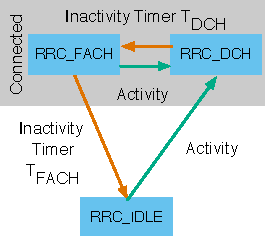
\includegraphics{network/background/figures/three_states}
	\caption{Three State Scenario}\label{fig:network:background:rrc_state_machines:three_states}
	\end{subfigure}
	\begin{subfigure}[b]{.5\textwidth}
	\centering
	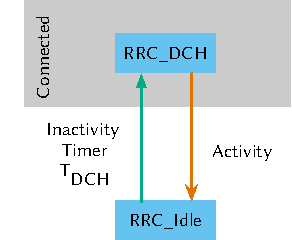
\includegraphics{network/background/figures/two_states}
	\caption{Two State Scenario}\label{fig:network:background:rrc_state_machines:two_states}
	\end{subfigure}
	\caption{\headershortacr{RRC} State Machine Diagrams}\label{fig:network:background:rrc_state_machines}
\end{figure}

In the following, we consider two different state transition models, depicted in \reffig{fig:network:background:rrc_state_machines}, based on the \gls{RRC} protocol.
The first model includes the \gls{RRC_idle}, \gls{RRC_FACH}, and \gls{RRC_DCH} states is shown in \reffig{fig:network:background:rrc_state_machines:three_states} and is in the following called the three state model.
If the \gls{UE} is in the \gls{RRC_idle} state and activity is detected, i.e. a packet is sent or received, the connection transitions to \gls{RRC_DCH} state.
After each transmission a timer \gls{TDCH} is started and reset whenever a new packet is sent or received.
If the timer expires, the connection transitions to the \gls{RRC_FACH} state
Upon entering, the \gls{TFACH} timer is started.
If a new transmission occurs, the connection again transitions to the \gls{RRC_DCH} state.
If \gls{TFACH} expires, the connection transitions to \gls{RRC_idle} state.

The second model, denoted as the two state model, and shown in \reffig{fig:network:background:rrc_state_machines:two_states}, only includes the \gls{RRC_idle} and \gls{RRC_DCH} state.
If the \gls{UE} is in the \gls{RRC_idle} mode and a packet is sent or received, the connection transitions to the \gls{RRC_DCH} state. Once in \gls{RRC_DCH} mode, the \gls{TDCH} timer is started and it is reset whenever a new packet is sent or received.
If the timer expires, the \gls{UE} transitions back to \gls{RRC_idle} state.

While the three state model is closer to the specified \gls{RRC} protocol is similar to some proprietary \emph{Fast Dormancy} implementations used by \gls{UE} vendors.
In these Fast Dormancy implementations, the \gls{UE} tears down the connection to the network state as soon as no data is ready to be sent for a certain time, i.e., it forces the network to transition to \gls{RRC_idle} state.
In contrast to the three state model, there is no transition to the \gls{RRC_FACH} state.
If a device disconnects from the network by transitioning to the \gls{RRC_idle} state, it has to be reauthenticated before another transition to the \gls{RRC_DCH} state can occur.
This results in additional signalling traffic and causes more load on the network \cite{NSN2011} due to frequent re-establishments of the RRC connection.
These proprietary Fast Dormancy algorithms do not adhere to the \gls{RRC} specification \cite{GSM2010}, but nontheless exist in the real world and have been identified as possible causes for signalling storms.
The major reason for Fast Dormancy implementations is the decrease in power consumption on the \gls{UE}, since the transmission unit of the \gls{UE} consumes only \SIrange{1}{2}{\percent} of the energy in \gls{RRC_idle} state compared to the \gls{RRC_DCH} state.
Thus, both models warrant further investigation.

\subsection{Measurements of \headershortacr{RRC} Parameters and Optimisation of Resource Consumption}\label{sec:network:background:measurement_optimisation}

In the literature, the configuration of the inactivity timers used for the \gls{RRC} protocols have been investigated in detail.
In~\cite{Perala2009} a measurement tool for \gls{RRC} protocol states is presented. 
It is used to determine \gls{RRC} state transition parameters, channel setup delays, and paging delay by measuring the one-way round trip time of data packets.
The results are validated by monitoring the energy consumption in different \gls{RRC} states.
One outcome is that \gls{UMTS} network configurations vary significantly by network operator.
\gls{RRC_DCH} release timer as well as the inactivity timer value triggering transition to \gls{RRC_idle} state were measured.
The values range from \SI{1.2}{\second} for the \gls{RRC_DCH} release timer to more than one minute for the \gls{RRC_idle} timer.
Similar results are presented in~\cite{Qian2010a}.
Here, the observed values vary between \SI{5}{\second} and \SI{12}{\second}. 
Additionally, they also determined the exact \gls{RRC} state transitions for two networks such as \gls{RRC_idle} \(\rightarrow\) \gls{RRC_FACH} \(\rightarrow\) \gls{RRC_DCH} or \gls{RRC_idle} \(\rightarrow\) \gls{RRC_DCH} directly without transitioning through the \gls{RRC_FACH} state.
The \gls{3GPP} has released a technical report \cite{3GPP_22801} about the adverse impact of mobile data applications.
This report states that frequent connection re-establishments due to small data packets caused e.g. by status updates of social network or instant messaging apps can lead to problems of increased signalling load.
This highlights the importance of this topic.

Furthermore, there are papers that propose optimizing strategies that take the \gls{RRC} states into account. 
In~\cite{Qian2011} the impact of different application traffic patterns is studied to reveal resource usage in mobile networks.
By identifying packet bursts, they infer the \gls{RRC} states of the \gls{UE}.
Radio resources are quantified by channel occupation time and energy consumption.
They propose an algorithm that tries to optimize application traffic patterns by e.g. piggybacking, batching up data, or decreasing the update rate of an application.
The algorithm is evaluated for six applications, two news applications, Pandora streaming application, Google search, Tune-In radio and Mobelix. 
In~\cite{Qian2010b} also \gls{RRC} states are studied for network optimization.
The authors optimize the inactivity timers to allow a better resource utilization. 
They propose a application-to-network interface to avoid unnecessary timer periods after data transmission.

\subsection{Smartphone Power Consumption and \headershortacr{QoE}}\label{sec:network:background:energy_consumption_qoe}
Power consumption of the \gls{UE} varies according to the devices current \gls{RRC} state.
The power consumption caused by \gls{RRC_DCH} mode was measured at about \SIrange{600}{800}{\milli\watt}~\cite{Qian2011,Qian2010a}.
In \gls{RRC_FACH} mode, the consumption was measured at about \SIrange{400}{460}{\milli\watt} depending on the \gls{UE} and the network operator~\cite{Qian2010a}.
A precise measurement of the power consumption of different \gls{RRC} states is performed in~\cite{Qian2010a,Balasubramanian2009,Lee2004}. 
The authors report that the energy drain depends on two factors: 
\begin{enumerate*}
\item user interactions and applications 
\item platform hardware and software.
\end{enumerate*}

In \cite{Ickin2012} the authors performed a 4 week long study with 29 participants to identify factors influencing \gls{QoE} of mobile applications.
The study comprises
\begin{enumerate*}
\item data from context sensing software,
\item user feedback using an experience sampling method several times per day, and
\item weekly interviews of the participants.
\end{enumerate*}
To determine the factors of influence, the authors analyze the frequency of specific keywords in the interviews and the surveys.
They find that the term \emph{battery} has the highest frequency.
According to the authors this is reasonable since the battery efficiency has a strong impact on the user perceived quality, in particular when it the \gls{UE} is nearly discharged.
\section{Trade-Offs for Multiple Stakeholders in LTE}\label{sec:application:lte_video}

\newcommand{\bandwidth}{\ensuremath{b_W}\xspace}
\newcommand{\bitrate}{\ensuremath{b_R}\xspace}
\newcommand{\timeplayedback}{\ensuremath{t_p}}

\newcommand{\download}{Download\xspace}
\newcommand{\live}{Live\xspace}
\newcommand{\serviceprovisioning}{Provisioning\xspace}
\newcommand{\streaming}{Streaming\xspace}

\newcommand{\streamingstart}{\ensuremath{\sigma}\xspace}
\newcommand{\bufferlower}{\ensuremath{\theta}\xspace}
\newcommand{\buffersize}{\ensuremath{\Theta}\xspace}

\newcommand{\ton}{\(T_{\texttt{ON}}\)\xspace}
\newcommand{\tdrxinactivity}{\(T_{\texttt{I}}\)\xspace}

\newcommand{\shortdrx}{\texttt{Short DRX}\xspace}
\newcommand{\tshortdrx}{\(T_{\texttt{S}}\)\xspace}
\newcommand{\longdrx}{\texttt{Long DRX}\xspace}
\newcommand{\tlongdrx}{\(T_{\texttt{L}}\)\xspace}
\newcommand{\rrcconnected}{\texttt{RRC Connected}\xspace}
\newcommand{\tidle}{\(T_{\texttt{Idle}}\)\xspace}
\newcommand{\tonidle}{\(T^{\texttt{Idle}}_{\texttt{ON}}\)\xspace}
\newcommand{\rrcidle}{\texttt{RRC Idle}\xspace}
\newcommand{\tdrxidle}{\(T^{\texttt{Idle}}_{\texttt{\gls{DRX}}}\)\xspace}
\newcommand{\promotiondelay}{\(D_P\)\xspace}

\newcommand{\bandwidthdown}{b_d\xspace}
\newcommand{\timedownloaded}{\ensuremath{t_d}}

\newcommand{\power}{P\xspace}
\newcommand{\energyconsumption}{\ensuremath{E}\xspace}
\newcommand{\connectioncount}{\ensuremath{C}\xspace}

\newcommand{\factordown}{\ensuremath{\alpha}\xspace}
\newcommand{\powerbaseline}{\ensuremath{\beta}\xspace}

\newcommand{\userabortrv}{\ensuremath{A}\xspace}
\newcommand{\userabortpdf}{\ensuremath{a}\xspace}
\newcommand{\meanwastedtraffic}{\ensuremath{W}\xspace}

\newcommand{\timeunwatched}{\ensuremath{t_u}}
\newcommand{\videolength}{l\xspace}



\subsection{System Model}\label{sec:application:cloud_file_synchronisation:system_model}
This section first provides a general overview over the Dropbox service architecture and introduces the considered usecase.
Then, we propose the cloud storage model and metrics used in this analysis.
Finally, we discuss a set of scheduling mechanisms used to start the file synchronisation process. 

The authors of~\cite{Drago2012} provide a first study of the \dropbox architecture, which is schematically depicted in \reffig{fig:application:cloud_file_synchronisation:system_model:dropbox_architecture} and used as a basis for the model under study in the remainder of this section.

\begin{figure}
  \centering
  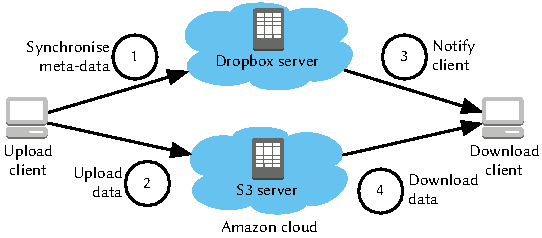
\includegraphics[width=\columnwidth]{application/cloud_file_synchronization/system_model/figures/dropbox_architecture}
  \caption{\dropbox file storage and retrieval process}
  \label{fig:application:cloud_file_synchronisation:system_model:dropbox_architecture}
\end{figure}

The \dropbox infrastructure consists of two main components:
\begin{enumerate*}
\item a storage cloud based on Amazon's Elastic Compute Cloud and Simple Storage Service, and 
\item (2) control servers directly maintained by \dropbox Inc. 
\end{enumerate*}

The control servers store meta information about the current state of the files in the \dropbox folders and trigger synchronization processes on the clients.

A file synchronization can basically be described in five steps.
As soon as the new file is added to the \dropbox folder of the uploading client, a preprocessing step is triggered and the meta information for the file are generated, respectively updated.
This information is then synchronized with the control servers~(1) and the file itself is uploaded to the storage cloud~(2).
After the file has completely been transferred to the storage cloud, all connected clients are notified about the update~(3) and start downloading the new file~(4).

\subsubsection*{Use Case: Photo Uploading}\label{sec:application:cloud_file_synchronisation:use_case}
In this section we consider the synchronization of images from a digital camera to a mobile \gls{UE} via a cloud storage provider.
Real world examples of this scenario are, e.g., taking photos of a live event and transferring them to a picture agency, or shooting private holiday images. 

The user took a finite set of pictures with a wearable device like Google Glass or a smart camera, e.g. a Nikon Coolpix S800c or SAMSUNG CL80.
The camera is then connected via a \gls{PAN} with a mobile \gls{UE}, for example a Laptop with a data card or a smartphone, to store the images on the mobile device.
The \gls{UE} uses broadband wireless Internet access technology and runs software provided by the cloud storage provider in order to synchronise the images with the cloud storage.
Finally, the scenario includes a remote client, which is connected using a wire line connection and downloads the images from the cloud.

For the evaluation presented in this paper, we consider a specific realization of the use case described above.
For the role of the cloud storage provider we consider \dropbox, Bluetooth is used as the technology for establishing the \gls{PAN}, and \gls{LTE} is used as the wireless broadband access technology.

In the considered scenario the interests of two stakeholders are impacted.
The first stakeholder, the end user, has two contradicting requirements on the system.
On the one hand side, the images should be synchronised as fast as possible. 
This requires a fast and permanent Internet connection of the \gls{UE}, which in turn is very power intensive.
On the other side, the power drain of the mobile device should be minimized to enable a long battery life time.
The second stakeholder, the mobile network provider, wants to minimize the signallisation overhead in the network~\cite{NSN2011, Huawei2011} caused by short time connections.
Here, an optimisation problem arises to find a practical solution for all three requirements. 
In order to analyse this problem, we use a simulation model of the file synchronization process, which is described in the following.

\subsubsection*{Cloud Storage Model and Performance Metrics}\label{sec:application:cloud_file_synchronisation:system_model:model_metrics}
The proposed simulation model is schematically depicted in \reffig{fig:application:cloud_file_synchronisation:system_model:model_metrics:model} and based on the findings of~\cite{Drago2012} described in~\refsec{sec:application:background}.

\begin{figure}
\centering
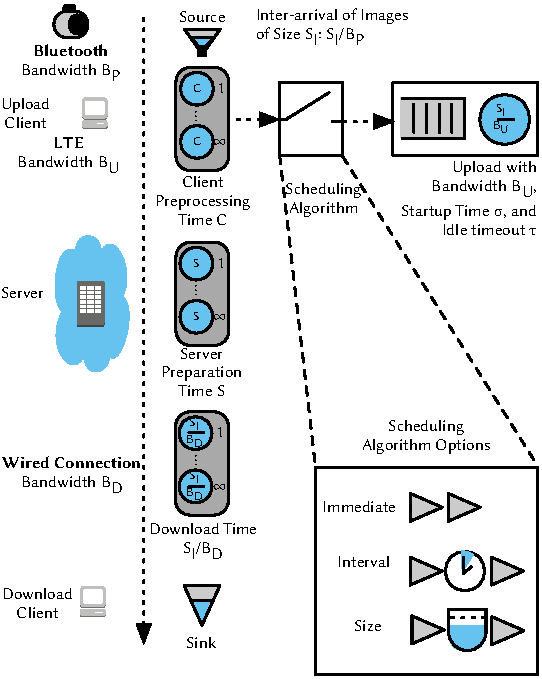
\includegraphics[width=\columnwidth]{application/cloud_file_synchronization/system_model/figures/model}
\caption{Synchronization Process Model}
\label{fig:application:cloud_file_synchronisation:system_model:model_metrics:model}
\end{figure}

We assume that the user has taken pictures of varying file size distributed with \imageFileSize.
These pictures are transfered from the camera to the mobile device using the \gls{PAN} with a constant bandwidth~\panTransferRate.
Due to the limited bandwidth \panTransferRate of the \gls{PAN} device, the inter-arrival times of images at the \dropbox shared folder of the mobile device can be calcluated by \(\interarrivaltime = \frac{\imageFileSize}{\panTransferRate}\).

As soon as the image is fully copied to the \dropbox folder, the generation of the meta data introduces a preprocessing delay, which we refer to as client preparation time~\clientpreparationtime.
To evaluate different strategies optimising the overall waiting time, power drain, and signallisation traffic we include a scheduling component.
This component implements different algorithms, described in \refsec{sec:application:cloud_file_synchronisation:system_model:algorithms}, which decide when the images currently held available in the scheduling component should be sent to the component responsible for transmission.

Next, we consider the \gls{LTE} \gls{UE} used for image upload.
Due to the specification of the \gls{LTE} standard \cite{3GPP_RRC_Spec}, the upload component can, at any point in time, either be connected to the mobile network or disconnected.
If the \gls{UE} is currently disconnected, and a new image for upload arrives, the connection process is triggered and completed after a startup delay \(\startupDelay = \SI{0.26}{\second}\).
Once the \gls{UE} is connected, arriving images are transmitted in order.
The transmission, i.e. service time, of an image depends on the size of the image currently being uploaded as well as the upload bandwidth \uploadbandwidth.
As only one image is transferred at once, waiting images are stored in a queue of infinite size.
If the \gls{UE} is idle for more than \(\idleThreshold = \SI{11.576}{\second}\), the device disconnects from the network.

After the image has been successfully uploaded to the storage servers, a server side preprocessing phase starts, before the file transfer to the downloading client starts.
This server side preprocessing again introduces an additional delay, the server preparation time~\serverpreparationtime, in the synchronization process.
Finally, the image is downloaded by the wire line client.
Again, the duration is calculated based on the size of the image and the available download bandwidth~\downloadbandwidth.

Next, we discuss the metrics used to evaluate the performance of the scheduling algorithms under consideration.
First, we consider the mean synchronization time \sojournTime, i.e., the time between the generation of images and the completion of the download.
This metric accounts for the desire of end users to synchronize images in a short amount of time.
Secondly, we study the relative amount of time the \gls{UE} is disconnected \relativeDisconnectedTime.
As the \gls{UE} consumes more power in the connected state, the user is generally interested in scheduling mechanisms which ensure that the device is only connected if required \cite{Ickin2012}.
This measure also enables a more general evaluation then the actually consumed power, as the concrete power drain differs significantly for each device.
Finally, we evaluate the number of transitions~\connectionCount between the connected and disconnected states.
As discussed in \refsec{chap:network}, frequent state transitions put a strain on the network due to increased signallling.
Thus, scheduling algorithms with a small number of transitions would be favored by network operators.

\subsubsection*{Scheduling Algorithms}\label{sec:application:cloud_file_synchronisation:system_model:algorithms}
We use different scheduling strategies in our model to control the uploading of the files from the mobile client.
These mechanisms in turn affect the synchronization time, the power drain, and the generated signalling traffic.

The most basic strategy of handing the upload is to immediately send new files, as soon as the meta data is generated.
We refer to this as \algoimmediate strategy and will use this as base line for all comparisons in the evaluations.
The other two strategies considered are based on a temporal, respectively a size threshold. 
Using the \algointerval scheduling, the client checks periodically if new files have been marked for synchronization.
If new files are present, they are synchronized to \dropbox.
Files which could not be sent within the current interval will automatically be added to the file batch for the next interval. 
The last scheduling mechanisms uses a threshold based on the overall \algosize of the images not yet synchronized.
If the threshold is crossed, an upload is triggered.

\subsection{Numerical Evaluation}\label{sec:application:lte_video:numerical_evaluation}

In this section we study the metrics introduced in \refsec{sec:application:lte_video:system_model:model_assumptions:metrics} on the different transmission mechanisms.

First, we study the impact of the considered transmission mechanisms on the energy consumption and the wasted traffic. 
Then, we consider the impact of the connection count for the \streaming mechanisms and varying values of the parameters \emph{stop threshold} \bufferlower and \emph{threshold size} \buffersize in more detail.

We consider a video of \(\videolength=\SI{1600}{\second}\) length which is viewed on a \gls{UE} with \gls{LTE} access.
The median of available downlink throughput in current \gls{LTE} networks is \(\bandwidth = \SI{12.74}{\mega\bit\per\second}\) \cite{Huang2012}.
A wide set of video bitrates between \SIlist{1;50}{\mega\bit\per\second} is in use~\cite{YouTube2013}.
In order to prevent stalling, we consider bitrates between \SIrange{1}{10}{\mega\bit\per\second}, staying below the available network bandwidth.
For the \streaming mechanism, a stop threshold of \(\bufferlower = \SI{4}{\second}\) and a threshold size of \(\buffersize = \SI{32}{\second}\) were selected.
Furthermore, we specify a prebuffering duration of \(\streamingstart = \SI{5}{\second}\).

We conduct our study using deterministic discrete event simulation which uses no random variables.
The wasted traffic is obtained analytically using the abort behaviour model.
Thus, all results are exact under the previously stated assumptions.

\subsubsection*{Energy Consumption}\label{sec:application:lte_video:numerical_evaluation:energy_consumption}
First, we study the influence of both video bitrate as well as the selected download mechanism on energy consumption in \reffig{fig:application:lte_video:numerical_evaluation:energy_consumption:bitrate2energy}.
\begin{figure}
  \centering
  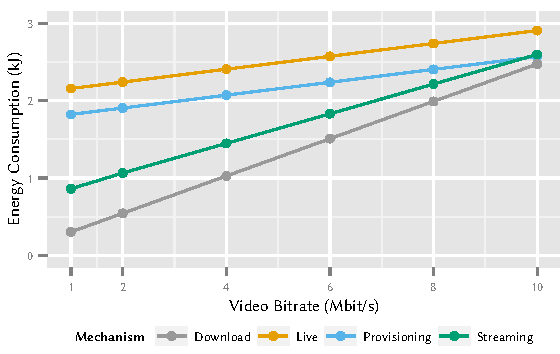
\includegraphics{application/lte_video/numerical_evaluation/figures/bitrate2energy}
  \caption{Influence of bitrate and download mechanism on energy consumption.}
  \label{fig:application:lte_video:numerical_evaluation:energy_consumption:bitrate2energy}
\end{figure}

We consider the \download mechanism and observe that it consumes the least amount of energy.
Here the video is downloaded with full bandwidth, as seen in \reffig{fig:application:lte_video:system_model:video_model}, resulting in a very short energy intensive download phase and a longer energy unintensive playback phase.
For the \live mechanism we observe the opposite, i.e. the highest energy consumption for all bandwidths.
If this mechanism is used, the used bandwidth equals the video bitrate.
Thus, the download requires the same amount of time as the playback, resulting in the highest possible energy consumption.
The \serviceprovisioning method uses a higher bandwidth, thus reducing the overall download time.
This reduced download time decreases the energy consumption when compared to the \live mechanism, even though the bandwidth used for downloading is increased to \SI{120}{\percent}.
For the \streaming mechanism we observe an energy consumption slightly higher than the \download mechanism.
As the bitrate of the video increases, the energy consumption increases as well.
This is due to the fact that a higher video bitrates require larger downloads.
For video bitrates approaching the available bandwidth the \streaming mechanism degenerates to the \live mechanism, as no prebuffering is possible.
We conclude that the \download and \streaming mechanisms outperform \live and \serviceprovisioning with regard to energy consumption.

\subsubsection*{Wasted Traffic}\label{sec:application:lte_video:numerical_evaluation:wasted_traffic}
Next, we consider the wasted traffic as a metric of the transmission mechanism quality.
If a user completely watches a video, no traffic is wasted, as all data downloaded is used during playback.
Thus, we consider only the cases where a user stops the playback before the video is finished.

\begin{figure}
  \centering
  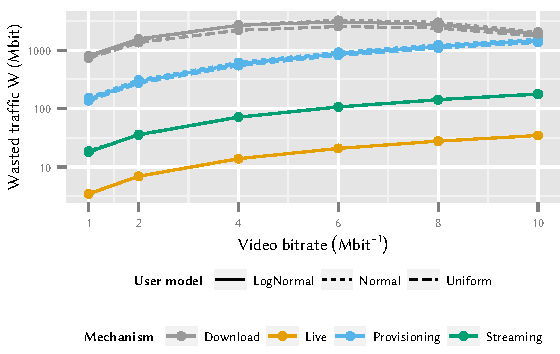
\includegraphics{application/lte_video/numerical_evaluation/figures/bitrate2lostData}
  \caption{Influence of bitrate, download mechanism and user model on wasted traffic. Download, Live, and Provisioning mechanisms result in equal connection counts.}
  \label{fig:application:lte_video:numerical_evaluation:energy_consumption:bitrate2lostData}
\end{figure}

In \reffig{fig:application:lte_video:numerical_evaluation:energy_consumption:bitrate2lostData} we study the wasted traffic for different video bitrates.
We consider the different transmission mechanisms introduced in \refsec{fig:application:lte_video:system_model:video_model} as well as the previously introduced user models.
We observe that the choice of user model has no significant impact on the wasted traffic.
For the \download mechanism, the amount of wasted traffic increases up to a video bitrate of \SI{6}{\mega\bit\per\second}, then the wasted traffic decreases as only video data which has been prebuffered can be lost if the user aborts the video.
As we assume an available bandwidth of \SI{12.74}{\mega\bit\per\second}, the bandwidth available for prebuffering decreases as the bitrate increases, resulting in lower amounts of wasted traffic for high video bitrates.
For the \live mechanism, we see that the wasted traffic for all user models is very low, but wasted traffic exists.
This is due to the traffic already sent by the server while the \gls{UE} is still waiting for promotion from \rrcidle to \rrcconnected, i.e. a short prebuffering phase exists.
As the bandwidth increases with the video bitrate, the wasted traffic increases as well.
Next, we consider the \serviceprovisioning approach and see an increase of wasted traffic as the video bitrate increases, due to the fact that the bandwidth used for continuous download is a factor of the video bitrate.
A higher video bitrate results in the download of the video being completed earlier, which leads to more wasted traffic.
Similar results can be seen for the \streaming mechanism, which results in more wasted traffic than the \live mechanism, but significantly less traffic than the \serviceprovisioning mechanism.
This is due to the fact that if the user aborts, at least the amount of video given by the \emph{stop threshold} \bufferlower and at most the complete buffer, given by the \emph{stop threshold} and the \emph{threshold size} are lost.
We have observed that the choice of user model results in no qualitative changes in wasted traffic.
As described in the last paragraph, the \download and \streaming mechanisms provide best results with regard to energy consumption.
However with regard to wasted traffic, the \live and \streaming mechanisms are most suited.
Thus, the \streaming mechanism seems to be a good compromise.
The network operator can select a tradeoff between energy consumption and wasted traffic as discussed in the next section.
From now on, we only consider the uniformly distributed user model.

\subsubsection*{Connection Count}\label{sec:application:lte_video:connection_count}
The \gls{ISP} is interested in reducing the number of connections occurring during video transmission.
Thus, we quantify the impact of the selected video transmission mechanism on the connection count, which directly correlates with the occurring signalling.

\begin{figure}
  \centering
  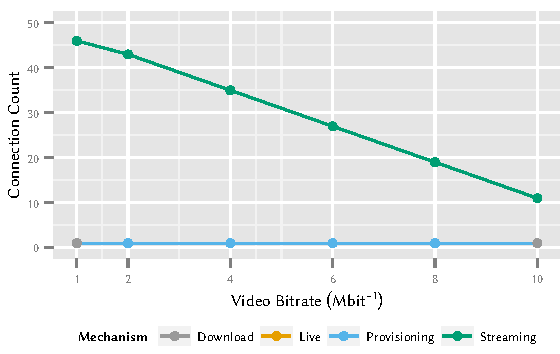
\includegraphics{application/lte_video/numerical_evaluation/figures/bitrate2connections}
  \caption{Influence of bitrate and download mechanism on connection counts.}
  \label{fig:application:lte_video:numerical_evaluation:energy_consumption:bitrate2connections}
\end{figure}

In \reffig{fig:application:lte_video:numerical_evaluation:energy_consumption:bitrate2connections} we study the impact of the different transmission mechanisms on the number of connections per transmission and thus the amount of generated signalling.
We observe that for the transmission mechanisms download, live, provisioning the number of connections is constantly one, independent of the selected bitrate \bitrate.
This is due to the fact that in these transmission mechanisms the video is transmitted in one chunk.
For streaming, the number of connections decreases as the video bitrate increases.
Here, a connection occurs each time the buffer is refilled.
For larger bitrates, refilling the buffer requires a longer transmission.
As the maximum time of video transmission is upper bounded by the video length, longer buffering phases result in a smaller total amount of buffering phases and thus in less connections per video transmission.

\begin{figure}
  \centering
  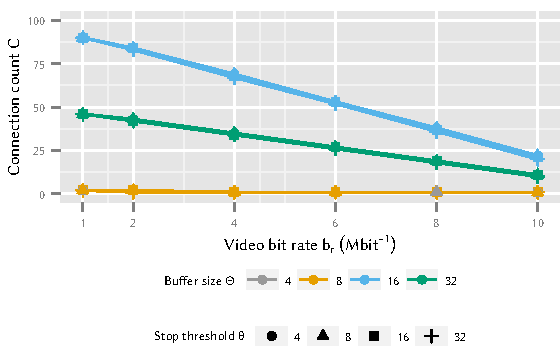
\includegraphics{application/lte_video/numerical_evaluation/figures/bitrate2connections_parameters}
  \caption{Influence of bitrate and selected parameters on connection counts for the streaming mechanism. Lines for different Stop Thresholds \(\theta\) overlap.}
  \label{fig:application:lte_video:numerical_evaluation:energy_consumption:bitrate2connections_parameters}
\end{figure}

Next, we consider the impact of the stop threshold~\bufferlower and buffer size~\buffersize on the number of connections \connectioncount caused by the \streaming mechanism.
In \reffig{fig:application:lte_video:numerical_evaluation:energy_consumption:bitrate2connections_parameters} we observe that while the buffer size has a significant impact on the number of connections during a video transmission, the lower buffer threshold has almost no impact.
For buffer sizes of \SIrange{4}{8}{\second}, no new connections are started, i.e. no signalling occurs.
This is due to the fact that the connection timeout in \gls{UE} is configured as \SI{11.576}{\second}, as discussed in \refsec{sec:application:lte_video:system_model:lte_network_model}.
Thus, for this low buffer sizes the \gls{UE} does not disconnect from the network.
Furthermore, we observe that as the buffer size increases, the number of connections decreases.
Refilling larger buffers requires, similar to larger bitrates, longer transmission times.
Thus, due to the total upper bound on the transmission time, less download phases can occur during the transmission.
\subsection{Trade-Offs}\label{sec:application:lte_video:trade_offs}
\subsubsection*{Transmission Mechanism Selection}\label{sec:application:lte_video:trade_offs:mechanism_selection}
\subsubsection*{Influence of Buffer Threshold Selection}\label{sec:application:lte_video:trade_offs:buffer_threshold_influence}

\begin{figure}
  \centering
  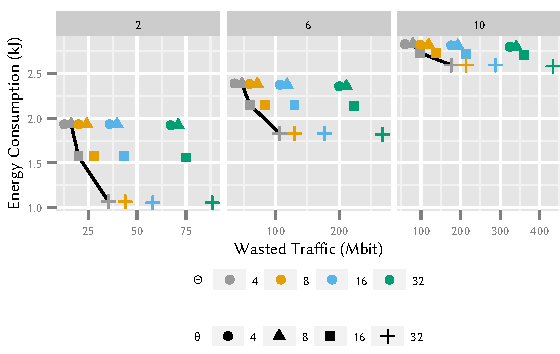
\includegraphics{application/lte_video/trade_offs/figures/energy2lostData}
  \caption{Evaluation of the streaming mechanism for varying video bitrates regarding energy consumption and wasted traffic}
  \label{fig:application:lte_video:numerical_evaluation:trade_offs:energy2lostData}
\end{figure}

\begin{figure}
  \centering
  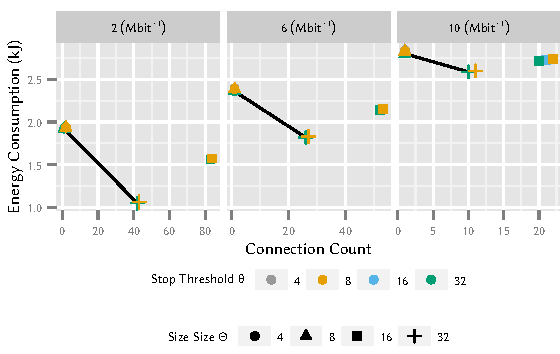
\includegraphics{application/lte_video/trade_offs/figures/energy2connections}
  \caption{Evaluation of the streaming mechanism for varying video bitrates regarding energy consumption and signalling}
  \label{fig:application:lte_video:numerical_evaluation:trade_offs:energy2connections}
\end{figure}

\begin{figure}
  \centering
  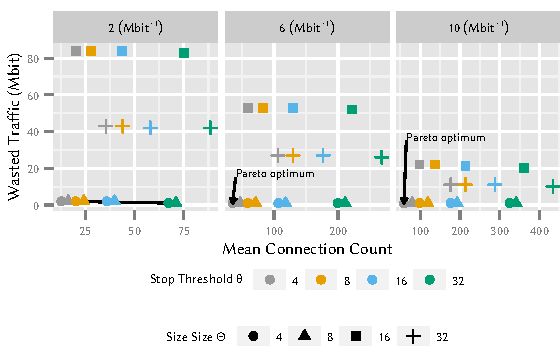
\includegraphics{application/lte_video/trade_offs/figures/connections2lostData}
  \caption{Evaluation of the streaming mechanism for varying video bitrates regarding signalling and wasted traffic}
  \label{fig:application:lte_video:numerical_evaluation:trade_offs:connections2lostData}
\end{figure} 
\section{Dimensioning Video Buffer for Specific User Profiles and Behavior}\label{sec:application:qoe_user_behaviour}

\newcommand{\stallingRatio}{\ensuremath{R}\xspace}
\newcommand{\stallingDuration}{\ensuremath{L}\xspace}
\newcommand{\numberStallingEvents}{\ensuremath{N^*}\xspace}
\newcommand{\stallingFrequency}{\ensuremath{F}\xspace}
\newcommand{\meanStallingEventDuration}{\ensuremath{L}\xspace}

\newcommand{\networkBandwidth}{\ensuremath{\lambda}\xspace}
\newcommand{\playbackRate}{\ensuremath{\mu}\xspace}

\newcommand{\meanBusy}{\ensuremath{B}\xspace}
\newcommand{\meanIdle}{\ensuremath{L}\xspace}
\newcommand{\numberFrames}{\ensuremath{Z}\xspace}
\newcommand{\videoDownloadTime}{\ensuremath{t_Z}\xspace}

\newcommand{\watchLater}{\emph{Watch Later}\xspace}
\newcommand{\watchNow}{\emph{Watch Now}\xspace}
\newcommand{\videoBrowsing}{\emph{Video Browsing}\xspace}

While the previous section implicitely assumed that sufficient bandwidth for video playback is available in order to provide high \gls{QoE}, this assumption on \gls{QoS} does not always hold in the real world, for example due to a high user count in the \gls{LTE} cell, or due to difficult terrain.
Traditional \gls{QoE} management mechanisms~\cite{Hossfeld2013c} consider a mapping function from \gls{QoS} to \gls{QoE} obtained from extensive user studies.
This \gls{MOS} homogenises different user ratings due to the use of an average, and do not consider the existence of user groups with distinct preferences.
In contrast to the earlier sections in this work, this sections considers tradeoffs between sub-groups of stakeholders, i.e. users with different playback preferences.

To this end, we first introduce models for video playback in \refsec{sec:application:qoe_user_behaviour:system_model}.
Then, we extend available \gls{QoE} models in order to support parameterisation for user preferences in \refsec{sec:application:qoe_user_behaviour:typical_user_scenarios:youtube_qoe}.
Finally, we evaluate a set of user scenarios in \refsec{sec:application:qoe_user_behaviour:typical_user_scenarios} using both the playback and the \gls{QoE} model.

\subsection{System Model}\label{sec:application:cloud_file_synchronisation:system_model}
This section first provides a general overview over the Dropbox service architecture and introduces the considered usecase.
Then, we propose the cloud storage model and metrics used in this analysis.
Finally, we discuss a set of scheduling mechanisms used to start the file synchronisation process. 

The authors of~\cite{Drago2012} provide a first study of the \dropbox architecture, which is schematically depicted in \reffig{fig:application:cloud_file_synchronisation:system_model:dropbox_architecture} and used as a basis for the model under study in the remainder of this section.

\begin{figure}
  \centering
  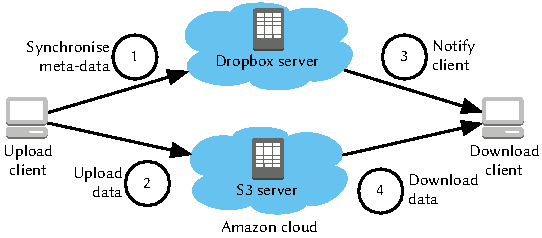
\includegraphics[width=\columnwidth]{application/cloud_file_synchronization/system_model/figures/dropbox_architecture}
  \caption{\dropbox file storage and retrieval process}
  \label{fig:application:cloud_file_synchronisation:system_model:dropbox_architecture}
\end{figure}

The \dropbox infrastructure consists of two main components:
\begin{enumerate*}
\item a storage cloud based on Amazon's Elastic Compute Cloud and Simple Storage Service, and 
\item (2) control servers directly maintained by \dropbox Inc. 
\end{enumerate*}

The control servers store meta information about the current state of the files in the \dropbox folders and trigger synchronization processes on the clients.

A file synchronization can basically be described in five steps.
As soon as the new file is added to the \dropbox folder of the uploading client, a preprocessing step is triggered and the meta information for the file are generated, respectively updated.
This information is then synchronized with the control servers~(1) and the file itself is uploaded to the storage cloud~(2).
After the file has completely been transferred to the storage cloud, all connected clients are notified about the update~(3) and start downloading the new file~(4).

\subsubsection*{Use Case: Photo Uploading}\label{sec:application:cloud_file_synchronisation:use_case}
In this section we consider the synchronization of images from a digital camera to a mobile \gls{UE} via a cloud storage provider.
Real world examples of this scenario are, e.g., taking photos of a live event and transferring them to a picture agency, or shooting private holiday images. 

The user took a finite set of pictures with a wearable device like Google Glass or a smart camera, e.g. a Nikon Coolpix S800c or SAMSUNG CL80.
The camera is then connected via a \gls{PAN} with a mobile \gls{UE}, for example a Laptop with a data card or a smartphone, to store the images on the mobile device.
The \gls{UE} uses broadband wireless Internet access technology and runs software provided by the cloud storage provider in order to synchronise the images with the cloud storage.
Finally, the scenario includes a remote client, which is connected using a wire line connection and downloads the images from the cloud.

For the evaluation presented in this paper, we consider a specific realization of the use case described above.
For the role of the cloud storage provider we consider \dropbox, Bluetooth is used as the technology for establishing the \gls{PAN}, and \gls{LTE} is used as the wireless broadband access technology.

In the considered scenario the interests of two stakeholders are impacted.
The first stakeholder, the end user, has two contradicting requirements on the system.
On the one hand side, the images should be synchronised as fast as possible. 
This requires a fast and permanent Internet connection of the \gls{UE}, which in turn is very power intensive.
On the other side, the power drain of the mobile device should be minimized to enable a long battery life time.
The second stakeholder, the mobile network provider, wants to minimize the signallisation overhead in the network~\cite{NSN2011, Huawei2011} caused by short time connections.
Here, an optimisation problem arises to find a practical solution for all three requirements. 
In order to analyse this problem, we use a simulation model of the file synchronization process, which is described in the following.

\subsubsection*{Cloud Storage Model and Performance Metrics}\label{sec:application:cloud_file_synchronisation:system_model:model_metrics}
The proposed simulation model is schematically depicted in \reffig{fig:application:cloud_file_synchronisation:system_model:model_metrics:model} and based on the findings of~\cite{Drago2012} described in~\refsec{sec:application:background}.

\begin{figure}
\centering
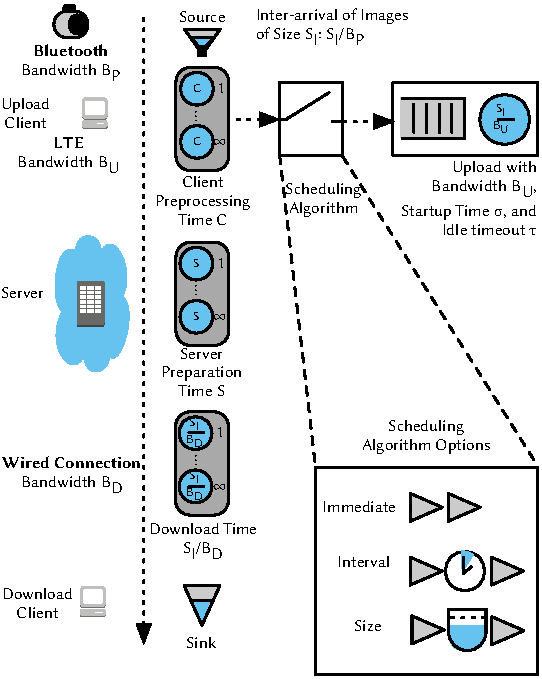
\includegraphics[width=\columnwidth]{application/cloud_file_synchronization/system_model/figures/model}
\caption{Synchronization Process Model}
\label{fig:application:cloud_file_synchronisation:system_model:model_metrics:model}
\end{figure}

We assume that the user has taken pictures of varying file size distributed with \imageFileSize.
These pictures are transfered from the camera to the mobile device using the \gls{PAN} with a constant bandwidth~\panTransferRate.
Due to the limited bandwidth \panTransferRate of the \gls{PAN} device, the inter-arrival times of images at the \dropbox shared folder of the mobile device can be calcluated by \(\interarrivaltime = \frac{\imageFileSize}{\panTransferRate}\).

As soon as the image is fully copied to the \dropbox folder, the generation of the meta data introduces a preprocessing delay, which we refer to as client preparation time~\clientpreparationtime.
To evaluate different strategies optimising the overall waiting time, power drain, and signallisation traffic we include a scheduling component.
This component implements different algorithms, described in \refsec{sec:application:cloud_file_synchronisation:system_model:algorithms}, which decide when the images currently held available in the scheduling component should be sent to the component responsible for transmission.

Next, we consider the \gls{LTE} \gls{UE} used for image upload.
Due to the specification of the \gls{LTE} standard \cite{3GPP_RRC_Spec}, the upload component can, at any point in time, either be connected to the mobile network or disconnected.
If the \gls{UE} is currently disconnected, and a new image for upload arrives, the connection process is triggered and completed after a startup delay \(\startupDelay = \SI{0.26}{\second}\).
Once the \gls{UE} is connected, arriving images are transmitted in order.
The transmission, i.e. service time, of an image depends on the size of the image currently being uploaded as well as the upload bandwidth \uploadbandwidth.
As only one image is transferred at once, waiting images are stored in a queue of infinite size.
If the \gls{UE} is idle for more than \(\idleThreshold = \SI{11.576}{\second}\), the device disconnects from the network.

After the image has been successfully uploaded to the storage servers, a server side preprocessing phase starts, before the file transfer to the downloading client starts.
This server side preprocessing again introduces an additional delay, the server preparation time~\serverpreparationtime, in the synchronization process.
Finally, the image is downloaded by the wire line client.
Again, the duration is calculated based on the size of the image and the available download bandwidth~\downloadbandwidth.

Next, we discuss the metrics used to evaluate the performance of the scheduling algorithms under consideration.
First, we consider the mean synchronization time \sojournTime, i.e., the time between the generation of images and the completion of the download.
This metric accounts for the desire of end users to synchronize images in a short amount of time.
Secondly, we study the relative amount of time the \gls{UE} is disconnected \relativeDisconnectedTime.
As the \gls{UE} consumes more power in the connected state, the user is generally interested in scheduling mechanisms which ensure that the device is only connected if required \cite{Ickin2012}.
This measure also enables a more general evaluation then the actually consumed power, as the concrete power drain differs significantly for each device.
Finally, we evaluate the number of transitions~\connectionCount between the connected and disconnected states.
As discussed in \refsec{chap:network}, frequent state transitions put a strain on the network due to increased signallling.
Thus, scheduling algorithms with a small number of transitions would be favored by network operators.

\subsubsection*{Scheduling Algorithms}\label{sec:application:cloud_file_synchronisation:system_model:algorithms}
We use different scheduling strategies in our model to control the uploading of the files from the mobile client.
These mechanisms in turn affect the synchronization time, the power drain, and the generated signalling traffic.

The most basic strategy of handing the upload is to immediately send new files, as soon as the meta data is generated.
We refer to this as \algoimmediate strategy and will use this as base line for all comparisons in the evaluations.
The other two strategies considered are based on a temporal, respectively a size threshold. 
Using the \algointerval scheduling, the client checks periodically if new files have been marked for synchronization.
If new files are present, they are synchronized to \dropbox.
Files which could not be sent within the current interval will automatically be added to the file batch for the next interval. 
The last scheduling mechanisms uses a threshold based on the overall \algosize of the images not yet synchronized.
If the threshold is crossed, an upload is triggered.

\subsection{YouTube \headershortacr{QoE} Model}\label{sec:application:qoe_user_behaviour:typical_user_scenarios:youtube_qoe}
This section introduces \gls{QoE} models for YouTube video playback.
First, we extend the \gls{QoE} mapping function introduced in~\cite{Hossfeld2013c} in order to support user preferences regarding sensitivity to stalling duration and number of stalling events.
Then, we provide a parametrised mapping function allowing for user preferences regarding initial delay.
Finally, we combine the proposed mapping functions.

\subsubsection*{Stalling \headershortacr{QoE} Model}\label{sec:application:qoe_user_behaviour:typical_user_scenarios:youtube_qoe:stalling}
The \gls{QoE} of \gls{HTTP} streaming depends mainly on the actual number of stalling events \(N\) for a video of duration \(T\) and the average length \(L\) of a single stalling event.
A \gls{QoE} model combining both key influence factors into a single equation \(f(L,N)\) is provided in~\cite{Hossfeld2013c} and found to follow the IQX hypothesis~\cite{Fiedler2010} describing an exponential relationship between the influence factors and \gls{QoE}.
In particular, the model function returns \gls{MOS} on a 5-point absolute category rating scale with 1 indicating the lowest \gls{QoE} and 5 the highest \gls{QoE}. 
\begin{equation}
 f(L,N) = 3.5 e^{-(0.15L + 0.19)N}+1.50
\label{eq:application:qoe_user_behaviour:typical_user_scenarios:youtube_qoe:stalling:original_model}
\end{equation}
Due to well known rating scale effects, the model in \refeq{eq:application:qoe_user_behaviour:typical_user_scenarios:youtube_qoe:stalling:original_model} has a lower bound of \(1.50\), as users avoid the extremities of the scale called \emph{saturation effect}, see e.g.~\cite{Moller2000}.
In contrast, if the video is not stalling, no degradation is observed and users rate the impact of stalling as 'imperceptible', i.e. a value of 5.

It has to be noted that the model function in \refeq{eq:application:qoe_user_behaviour:typical_user_scenarios:youtube_qoe:stalling:original_model} is based on subjective user studies with videos of duration up to \(T=\SI{30}{\second}\).
For other video durations, the normalized number \(N^*=\frac{N}{T}\) of stalling events has to be considered which requires to adapt the parameters \(\alpha=0.15\) and \(\beta=0.19\) in \refeq{eq:application:qoe_user_behaviour:typical_user_scenarios:youtube_qoe:stalling:original_model}, respectively. 

As the goal of our investigation is the analysis of the impact of different user profiles, we parametrize the function in \refeq{eq:application:qoe_user_behaviour:typical_user_scenarios:youtube_qoe:stalling:original_model} with parameters \(\alpha\) and \(\beta\) and conduct a parameter study on their impact. 
For the sake of simplicity, we normalize the QoE value to be in the range \(\left[0;1\right]\)  and use the normalized number of stalling events $N^*$. 
As a result, we arrive at \refeq{eq:application:qoe_user_behaviour:typical_user_scenarios:youtube_qoe:stalling:parameterized_model} as parametrized \gls{QoE} model \(Q_1\) to quantify the impact of stalling on QoE for different user profiles expressed by \(\alpha\) and \(\beta\). 
Thereby, the parameter \(\alpha\) adjusts the sensitivity of the user to the stalling duration \(L\cdot N^*\), while \(\beta\) quantifies the sensitivity of the user to the actual number of stalling events, i.e. the video interruptions.
Therefore, we will also use the term \emph{duration parameter} and \emph{interruption parameter} for \(\alpha\) and \(\beta\), respectively.

\begin{equation}
   Q_1(L,N^*) = e^{-\left( \alpha L + \beta\right) N^*} 
\label{eq:application:qoe_user_behaviour:typical_user_scenarios:youtube_qoe:stalling:parameterized_model}
\end{equation}

The model function \(Q_1\) in \refeq{eq:application:qoe_user_behaviour:typical_user_scenarios:youtube_qoe:stalling:parameterized_model} has the same form as \refeq{eq:application:qoe_user_behaviour:typical_user_scenarios:youtube_qoe:stalling:original_model} and follows the IQX hypothesis, but allows to investigate different user profiles.
For example, some users may suffer stronger from interruptions which is then adjusted by a higher value of \(\beta\).
Thus, a user profile can be expressed in terms of different values of the duration parameter \(\alpha\) and the interruption parameter \(\beta\)

\subsubsection*{Initial Delay \headershortacr{QoE} Model}\label{sec:application:qoe_user_behaviour:typical_user_scenarios:initial_delay}
Another impairment on \gls{HTTP} streaming \gls{QoE} are initial delays before the video playout can start for the first time.
The impact of initial delays \(T_0\) is modeled by the function given in \refeq{eq:application:qoe_user_behaviour:typical_user_scenarios:initial_delay:original_model}, model parameters are obtained from subjective tests \cite{Hossfeld2012c}. 
\begin{equation}
g(T_0)=-0.963 \mathrm{log10}(T_0 + 5.381) + 5
\label{eq:application:qoe_user_behaviour:typical_user_scenarios:initial_delay:original_model}
\end{equation}

The results in~\cite{Hossfeld2012c} show that the impact of the initial delay is independent of the video duration which was either \SI{30}{\second} or \SI{60}{\second} in the user tests.
Further, it was observed that users have a clear preference of initial delays instead
of stalling and that service interruptions have to be avoided in any case, even at costs of increased initial delays for filling up the video buffers. 

For the sake of simplicity, we normalize the function in \refeq{eq:application:qoe_user_behaviour:typical_user_scenarios:initial_delay:original_model} to obtain the \gls{QoE} model \(Q_2\) for initial delays \(T_0\), so that \(Q_2\) returns values in \(\left[0;1\right]\) and that \(Q_2(0)=1\) holds, by adding the term \(\gamma \mathrm{log10}\left(c\right)\).

The user profile is parametrized with the parameter \(\gamma\) determining the impact of initial delays on the user \gls{QoE}.
The constant \(c=5.381\) is taken from \refeq{eq:application:qoe_user_behaviour:typical_user_scenarios:initial_delay:original_model} defining the shape of the curve. 
Since the logarithm is not bounded, only positive values are considered to ensure \(Q_2(T_0) \in [0;1]\).
\begin{equation*}
Q_2(T_0)= -\gamma \mathrm{log10}\left(T_0 + c\right) + \gamma \mathrm{log10}\left(c\right)+ 1 
\end{equation*}

\subsubsection*{Combined \headershortacr{QoE} Model}\label{sec:application:qoe_user_behaviour:typical_user_scenarios:youtube_qoe:combined}
For dimensioning the video buffers, we are interested in a \gls{QoE} model which considers both, the impairments due to stalling and due to initial delays of the video playout.
However, to the best of our knowledge no combined model exists so far which has been validated by proper subjective user studies.
Therefore, we suggest the following model \(Q\).
Since the impact of stalling events clearly dominates the user perception \cite{Hossfeld2012a,Hossfeld2012c}, we consider the following rationale for the combined QoE model.
A user facing an initial delay \(T_0\) experiences a \gls{QoE} value of \(Q_2(T_0)\).
If additional stalling events occur, this will lower the QoE further.
Thus, \(Q_2(T_0)\) is the upper bound of \gls{QoE}.
For \(N^*\) stalling events with an average length \(L\), the \gls{QoE} will be further decreased by \(Q_1(L,N^*)\).

An additive \gls{QoE} model for non-adaptive HTTP streaming which is referred to as buffer-related perceptual indicator is recommended in \cite{ITUT2012}. This model follows the same rationale above, start from the maximum QoE value which is \(1=Q(0,0,0)\), subtract the degradation from stalling \(1-Q_1(L,N^*)\) and \(1-Q_2(T_0)\) stemming from initial delay.

Then, we arrive at the following additive QoE model \(Q\) used in the following analysis.  
\begin{eqnarray}
  Q(T_0,L,N^*) &=& 1-(1-Q_1(L,N^*)) - (1-Q_2(T_0)) \notag\\
   &=& Q_1(L,N^*) + Q_2(T_0) - 1
\label{eq:application:qoe_user_behaviour:typical_user_scenarios:youtube_qoe:combined:qsum}
\end{eqnarray}

\subsection{\headershortacr{QoE} Study for Typical User Scenarios}\label{sec:application:qoe_user_behaviour:typical_user_scenarios}
Based on the playback model introduced in \refsec{sec:application:qoe_user_behaviour:system_model} and the parametrised \gls{QoE} user model proposed in \refsec{sec:application:qoe_user_behaviour:typical_user_scenarios:youtube_qoe}, this section studies three typical user scenarios.
We discuss optimal choices for buffer size depending on user preferences and highlight the impact of buffer choices neglecting the user preference.

\subsubsection*{Watch later Scenario}\label{sec:application:qoe_user_behaviour:typical_user_scenarios:watch_later}
In the \watchLater scenario, a user requests a video, but the user does not expect that the video playout starts immediately. 
This may be the case for example when the user wants to watch an HD at a later time and expects low network bandwidth. 
During that initial delay, the user may opt do something else, e.g. opening another web page in a parallel tab in the browser.
Thus, \gls{QoE} is not affected by initial delays and we only need to consider \(Q_1\) in \refeq{eq:application:qoe_user_behaviour:typical_user_scenarios:youtube_qoe:stalling:parameterized_model}.

In the steady state, we have \(L=\frac{d}{\lambda}\) and \(N^*=\frac{\mu-\lambda}{d}\) and we obtain the following QoE relation in \refeq{eq:application:qoe_user_behaviour:typical_user_scenarios:stalling_steady_state}. 

\begin{equation}
   Q_1(L,N^*) = e^{\left(\mu-\lambda\right)(\frac{\alpha}{\lambda} +\frac{\beta}{d^*})}
	 = e^{-\alpha \frac{1-a}{a} - \beta \frac{1-a}{d^*}}
\label{eq:application:qoe_user_behaviour:typical_user_scenarios:stalling_steady_state}
\end{equation}

Since the \gls{QoE} function in \refeq{eq:application:qoe_user_behaviour:typical_user_scenarios:stalling_steady_state} is strictly monotonically increasing in the normalized buffer size \(d^*\), the optimum is achieved for 
\[Q_+=\lim\limits_{d^* \to \infty} Q_1(L,N^*)=e^{-\alpha \frac{1-a}{a}}.\]
Thus, the QoE value only depends on the parameter \(\alpha\) in the limit.
To see for which buffer size we are close to the optimum, we consider the relative difference \(\frac{Q_+-Q_1(L,N^*)}{Q_+}\) when it is less than \(\Omega=\SI{5}{\percent}\).
This is true for any \(d^*> -\beta \frac{1-a}{\log\left(1-\Omega\right)}\). 

For \(\beta \in \{0.05,0.2\}\), a small buffer size of \(d^*>\SI{4}{\second}\) is already sufficient to be close to the optimum \(Q_+\) for any offered network condition \(a\).
For users extremely sensitive to stalling, e.g. for \(\beta=0.8\), buffer sizes up to \SI{15}{\second} are required.
However, a buffer of \SI{4}{\second} is sufficient for a relative difference to the optimum of \SI{20}{\percent}. 
In general, the larger the buffer size the better the obtained \gls{QoE} is in this scenario. In practice, a buffer size of \SI{4}{\second} is a good choice.

\subsubsection*{Default Video Streaming Scenario}\label{sec:application:qoe_user_behaviour:typical_user_scenarios:default}

In the case of normal streaming, the user wants to watch a video immediately for a long period of time.
In contrast to the \watchLater scenario, the initial delay impacts the \gls{QoE} in the \watchNow scenario according to \refeq{eq:application:qoe_user_behaviour:typical_user_scenarios:youtube_qoe:combined:qsum}.

\begin{figure}
  \centering
  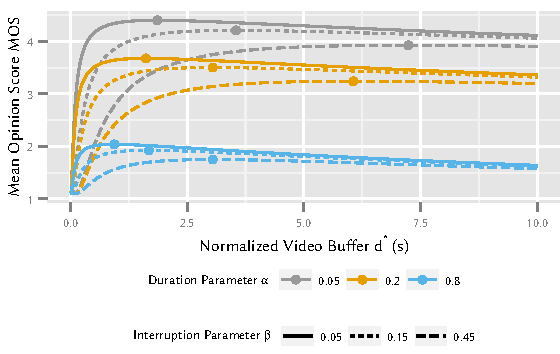
\includegraphics{application/qoe_user_behaviour/user_scenarios/figures/default_scenario}
  \caption{Dimensioning of buffer size in the \emph{Streaming Scenario} for available network bandwidth of \(a = 0.5\). Maxima marked as dots mainly depend on \(\beta\).}
  \label{fig:application:qoe_user_behaviour:typical_user_scenarios:default:default_scenario}
\end{figure}

\reffig{fig:application:qoe_user_behaviour:typical_user_scenarios:default:default_scenario} shows \gls{QoE} depending on the buffer size \(d^*\) for the \watchNow scenario and different user profiles in a network situation \(a=0.5\) leading to a stalling ratio \(R=0.5\).

Now, \gls{QoE} optima exist for finite buffer size, if the impact of the initial delay is taken into consideration. 
We notice that \(\alpha\) does increase the \gls{QoE} but has no significant impact on the optimal buffer size.
In contrast, for different \(\beta\) we observe different optima for the buffer size.
Therefore, we can neglect the interruption parameter \(\alpha\) when optimising the buffer size with regard to the \gls{QoE}.
A buffer size less than \SI{0.5}{\second} results in a severe loss of \gls{QoE} for all users.
A buffer size of \SIrange{2}{4}{\second} offers a good \gls{QoE} for the average user and any sensitive user.
Increasing the buffer size further decreases the \gls{QoE}.

\subsubsection*{Video Browsing Scenario}\label{sec:application:qoe_user_behaviour:typical_user_scenarios:browsing}

In the case of the \videoBrowsing scenario, the user watches a video for a short period of time. This includes cases such as, viewing a short video completely, viewing a short part of a long video or skipping ahead in a video frequently, thus watching multiple short parts of a video.
In this scenario, a steady state can not be assumed due to the short watching duration.
Since we know from the previous section that \(\alpha\) and \(\beta\) have only a marginal impact on the optimal \gls{QoE}, we consider only the default parameters \(\alpha=0.15\) and \(\beta=0.2\) in the following.
However, for video browsing, the impact of the initial delay may be more important for the user. Therefore, we consider two different types of delay sensitive users with \(\gamma=0.2\) as well as a more delay sensitive user with \(\gamma=0.8\).

\begin{figure}
  \centering
  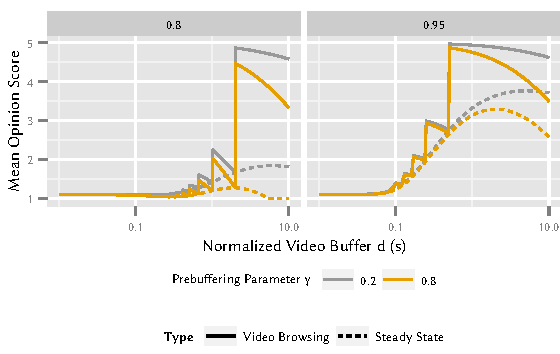
\includegraphics{application/qoe_user_behaviour/user_scenarios/figures/video_browsing}
  \caption{Dimensioning of buffers for \emph{Video Browsing} users with varying \gls{QoE} sensitivity to initial delays. Users abort the video after \SI{10}{\second}.}
  \label{fig:application:qoe_user_behaviour:typical_user_scenarios:browsing:video_browsing}
\end{figure}

In \reffig{fig:application:qoe_user_behaviour:typical_user_scenarios:browsing:video_browsing}, the impact of the buffer size on the \gls{QoE} is depicted for the case that the video is aborted after the first \SI{10}{\second} using a logarithmic x-axes. 
We consider two different network scenarios with an offered load of \(a = 0.8\) and \(a = 0.9\).
Multiple local QoE maxima exist independently of \(\gamma\), which appear when the number of stalling events change. 
For different values of \(\beta\) these maxima occur at the same buffer size.
Therefore, we can ignore \(\beta\) in this scenario. 
The local minima exist at the buffer size for which the last stalling event has the smallest possible length. 
The results for the steady state are also included and we observe that the steady state provides a lower bound for the finite buffer results.

Thus, the steady state can be used to perform worst case buffer dimensioning.
For very low offered loads \(a\), e.g. \(a = 0.1\) which is not shown due to scale, the \gls{QoE} is very low for both, the steady state and the finite case. 
Thus, video streaming and especially \videoBrowsing is not desirable in this case. 
However, for larger buffer sizes, the difference between the local maxima and the steady state increases. 
Nevertheless, in those cases, the initial delay exceeds tens of seconds.
So this scenario can not be described as realistic \videoBrowsing.

In general, if the exact viewing length of a video was known, e.g. short videos will be watched completely, the buffer size could be set so that the \gls{QoE} lies at a local maximum which is independent of \(\gamma\).
However, this method can result in a severe loss of \gls{QoE}, depending on \(\gamma\) if the user aborts earlier, as the actual \gls{QoE} loss significantly depends on \(\gamma\). 
In practice, a buffer size of \SIlist{1;2}{\second} is recommended for video browsing. 
If the buffer size is set too large, \(\gamma\) determines again the actual \gls{QoE} loss.
For larger buffer sizes, the sensitivity \(\gamma\) to initial delays strongly influence the \gls{QoE}.
\section{Cloud File Synchronization Services}
\cite{Schwartz2014a}

\subsection{System Model}
\subsubsection*{Use Case: Photo Uploading}
\subsubsection*{Cloud Storage Model and Performance Metrics}
\subsubsection*{Scheduling Algorithms}

\subsection{Measurement}
\subsubsection*{Bandwidth and Preparation Times}
\subsubsection*{Image File Sizes}

\subsection{Numerical Evaluation}
\subsubsection*{Waiting Time}
\subsubsection*{Relative Disconnection Time}
\subsubsection*{Connection Count}
\subsubsection*{Mechanism Comparison}
\subsubsection*{Trade-off Analysis}
\section{Lessons Learned}\label{sec:network:lessons_learned}
In this chapter we studied the impact of smartphone application traffic on mobile communication networks.
We considered three stakeholders interacting in the mobile network.
The \emph{mobile network operator} is interested in preventing so called signalling storms, where network components performance is degraded due to high signalling load caused by applications generating network traffic from users' \glspl{UE}.
The \emph{hardware vendor} is interested in satisfying customers by providing a long battery lifetime for the \gls{UE}, i.e. reducing power drain.
The \emph{application developer} is interested in increasing \gls{QoE} for the applications user.
Each of the stakeholders can influence the mobile network, by manipulating the parameters under its control.
The network operator can manipulate \gls{RRC} timers, increasing the time a smartphone stays connected to the network if no data is sent or received, decreasing the number of connections being established or severed and thus the signalling load in the network. 
The hardware vendor can implement proprietary \gls{RRC} protocol extensions, skipping power intensive connection states in order to reduce power drain.
The application developer can shorten update intervals, in order to provide more up to date events and increase \gls{QoE}.
However, each of the parameters under control of the individual stakeholders influence the \glspl{KPI} of the other stakeholders.

This chapter provides a two-pronged approach to analysing the impact of changes by individual stakeholders on the overall network.

First, we provided an algorithm to derive \gls{RRC} state transitions from traffic measurements of already deployed or prototyped applications.
While proprietary mechanisms exist to directly measure \gls{RRC} state transitions, due to the high price they are usually out of reach for application developers, preventing them from evaluating the impact of their applications on the network.
Based on this algorithm we analyse four popular smartphone applications, and find that while it is possible to find a viable tradeoff between signalling load and power drain for single applications, no such tradeoff exists if multiple applications operating in the network at the same time are considered.
For example, for the considered \emph{Twitter} application, increasing the network timer \TDCH from \SI{10}{\second} to \SI{11}{\second} would result in a decrease of signalling by \SI{40}{\percent}, while only resulting in an increase of power drain of \SI{6}{\percent}.
However, if the \emph{Aupeo} application is running in the same network optimised for the Twitter application, this change results in no reduction of signalling load and an increased power drain of \SI{5}{\percent}. 

Furthermore, we show that network timer optimisation, a practice where network operators manipulate \gls{RRC} timers in order to reduce signalling load, incentivises users to enable proprietary fast dormancy algorithms, resulting in a net increase of signalling load.
For example, if a network operator increases the \TDCH network timer from \SI{4}{\second} to \SI{8}{\second}, in order to reduce the signalling frequency caused by the Angry Birds application by \SI{67}{\percent}, this results in an increased power drain at the user's \gls{UE} of \SI{341}{\percent}.
If the user enables the fast dormancy option of the \gls{UE}, the power drain is decreased by \SI{27}{\percent}, however this increases the signalling frequency above the original value before the reconfiguration of the network operator.
%We also show that while longer \gls{RRC} timers may have an adverse effect on power drain due to the smartphone being longer connected to the network, it results in an increase of Web \gls{QoE}, as this results in web pages being able to be loaded faster if the smartphone is already connected to the network.

Second, we propose an analytical model to derive the \glspl{KPI} from analytical or empirical traffic distributions, in order to evaluate the impact of applications that do not yet exist or classes of applications defined by a common traffic characteristics.
Our results show that different access patterns have a considerable impact on the required resources of the mobile phone and the network.
We identified bursty traffic pattern as particularly resource-efficient with respect to power drain and signalling load.
In contrast, nearly periodic traffic is likely to cause signalling overload due to frequent connection re-establishments, especially when the connection timeout is slightly below the inter-packet time.
This can be observed on the example of a \TDCH timer of \SI{10}{\second}.
Here, the coefficient of variation has no impact on the signalling load for very small inter-packet times \(E[\PacketIAT]<\SI{1e-1}{\second}\) or very large inter-packet times \(E[\PacketIAT]>\SI{1e3}{\second}\).
For example, for a mean inter-arrival time of \(E[\PacketIAT] = 11.5\) seconds, an increase of coefficient of variation from \(0.5\) to \(5.0\) can decrease the signalling load by \SI{53}{\percent}.

Concluding from this chapter, we see that in mobile networks many different players, metrics, and tradeoffs exist.
We highlighted one examples of such a tradeoff, i.e. signalling load vs. power drain and discussed the influence of the current optimisation parameters, the network timers, on another.
However, many additional tradeoffs exist.
For example, the mobile operator has to balance the use of radio resources with the number of generated signalling frequencies.
Furthermore, application providers seek to improve the user experience which usually result in a higher frequency of network polls, creating additional signalling traffic.
The high number of tradeoffs and involved actors in this optimisation problem indicate that the current optimisation technique used by operators is no longer sufficient.

Approaches like \emph{Economic Traffic Management}~\cite{spirou2009} or \emph{Design for Tussle}~\cite{trilogy2008} could be applied to find
an acceptable tradeoff for all parties.
In Economic Traffic Management all participating entities share information in order to enable collaboration.
This collaboration allows for a joint optimisation of the tradeoff.
Design for Tussle aims to resolve tussles at run time, instead instead of design time.
This prevents the case that one actor has full control over the optimisation problem, which would likely result in the actor choosing a tradeoff only in its favour, ignoring all other participants.
One example of an actor providing information for another in order to optimise the total system would be \gls{UE} vendor providing interfaces for application developers to use when sending data.
These interfaces would schedule data to be transmitted in such a way that signalling load and power drain would be reduced, if the application’s requirements allow for it.
Until such interfaces exist, application developers could take the effect of the traffic their applications
produce both on the \gls{UE} and the network into account, for example using the algorithms proposed in this chapter. 